%!TEX root = featurecalc.tex
\subsection{Horizontal Cross-section Area}
\label{ssec:methodology:hca}

When 3D ROI is examined in a contour view as shown in Figure ~\ref{fig:methodology:roicontour}, it is obvious that the regions of different given depth ranges can be used to describe a sample.

\begin{figure}[htb]
\begin{center}
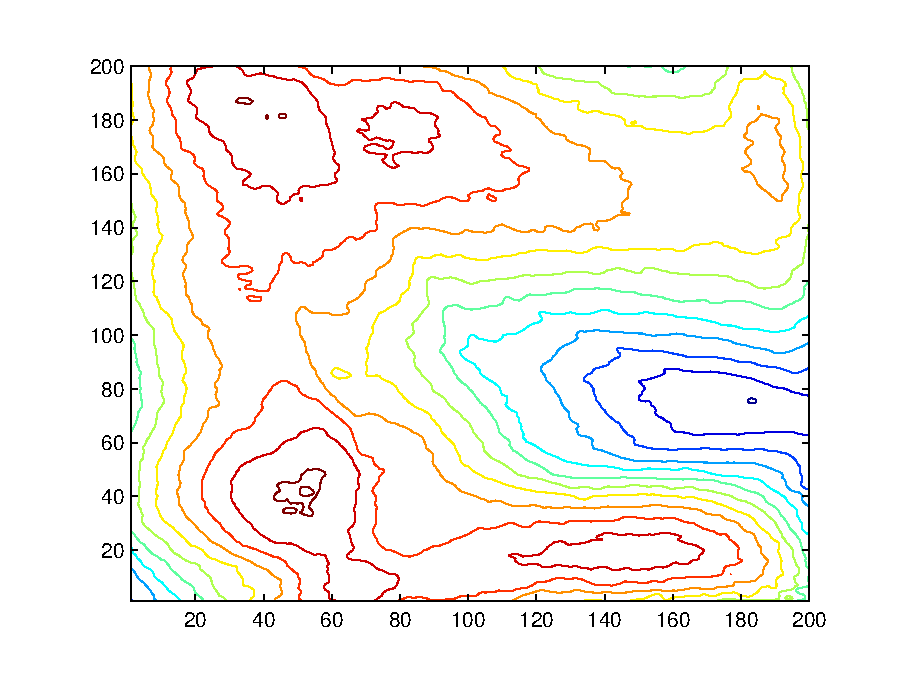
\includegraphics[width=0.9\linewidth]{ch-methodology/figures/roicontour}
\caption[Contour view of a 3-D ROI]{Contour view of a 3-D ROI}
\label{fig:methodology:roicontour}
\end{center}
\end{figure}

A group of equidistant horizontal planes cut the 3D ROI as shown in Figure ~\ref{fig:methodology:planecut}. Figure ~\ref{fig:methodology:roicontour} shows that most of the deeper level (enclosed with blue curves) are connected. These are more stable in response to noise or transformation.

\begin{figure}[htb]
\begin{center}
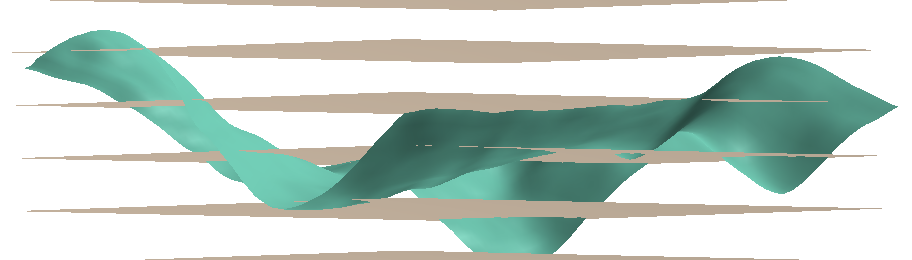
\includegraphics[width=0.9\linewidth]{ch-methodology/figures/planecut}
\caption[3D ROI cut by parallel horizontal planes]{3D ROI cut by parallel horizontal planes}
\label{fig:methodology:planecut}
\end{center}
\end{figure}


To get a stable HCA, we take into consideration only the levels from the deepest point to the reference plane, defined in Section ~\ref{ssec:methodology:md}. Suppose we divide this region into $N$ levels. Every level $G^k, k=1,2,\dots,N$ is described with a 200 by 200 matrix and calculated as

\begin{equation}
G^k_{ij} =
\begin{cases}
1 & \text{if} d_{ij}>h\cdot(N-k+1)/N,\\
0 & \text{otherwise}
\end{cases}
k=1,2,\dots,N;i=1,2,\dots,200;j=1,2,\dots,200;
\end{equation}

where $d_{ij}$ is the depth value of the $i^{th}$ row and $j^{th}$ column pixel of the ROI defined in ~\ref{eq:methodology:roimatrix} and $h$ is the palmprint depth defined by ~\ref{eq:methodology:md}.

To stabilize the areas, the growth of higher level is constrained to its previous level except the first level. That is

\begin{equation}
L^k=
\begin{cases}
G^1                             & k=1 \\
G^k \cap (L^{k-1} \oplus \Theta^{k-1}) & k=2,3,\dots,N
\end{cases}
\end{equation}

where $\cap$ denotes logical AND, $\oplus$ denotes a morphological dilation operation and  $\Theta^{k}$ is a disk morphological structuring element whose size can be calculated by $35-3 \times k$ (which is suitable for N = 8 by experience).

\begin{figure}[htb]
\begin{center}
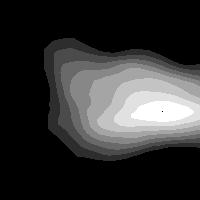
\includegraphics[width=0.9\linewidth]{ch-methodology/figures/hcastack}
\caption[$L^k$ shown stacked when $N=8$]{$L^k$ shown stacked when $N=8$}
\label{fig:methodology:hcastack}
\end{center}
\end{figure}

Figure ~\ref{fig:methodology:hcastack} shows an example of all the levels stacked together.

\begin{figure}[htb]
\centering
\subfigure[$k=1$]{
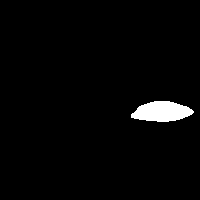
\includegraphics[height=0.18\textheight]{ch-methodology/figures/hca1-1}
\label{fig:methodology:hcalevels:1-1}
}\hspace{0.15\linewidth}
\subfigure[$k=2$]{
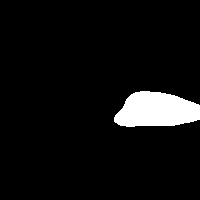
\includegraphics[height=0.18\textheight]{ch-methodology/figures/hca1-2}
\label{fig:methodology:hcalevels:1-2}
}\\
\subfigure[$k=3$]{
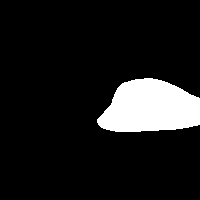
\includegraphics[height=0.18\textheight]{ch-methodology/figures/hca1-3}
\label{fig:methodology:hcalevels:1-3}
}\hspace{0.15\linewidth}
\subfigure[$k=4$]{
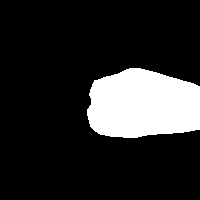
\includegraphics[height=0.18\textheight]{ch-methodology/figures/hca1-4}
\label{fig:methodology:hcalevels:1-4}
}\\
\subfigure[$k=5$]{
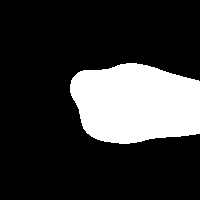
\includegraphics[height=0.18\textheight]{ch-methodology/figures/hca1-5}
\label{fig:methodology:hcalevels:1-5}
}\hspace{0.15\linewidth}
\subfigure[$k=6$]{
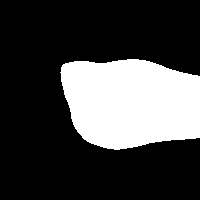
\includegraphics[height=0.18\textheight]{ch-methodology/figures/hca1-6}
\label{fig:methodology:hcalevels:1-6}
}\\
\subfigure[$k=7$]{
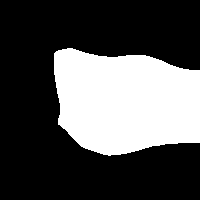
\includegraphics[height=0.18\textheight]{ch-methodology/figures/hca1-7}
\label{fig:methodology:hcalevels:1-7}
}\hspace{0.15\linewidth}
\subfigure[$k=8$]{
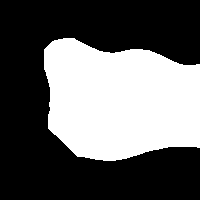
\includegraphics[height=0.18\textheight]{ch-methodology/figures/hca1-8}
\label{fig:methodology:hcalevels:1-8}
}
\caption[$L^k$ of one sample from palm 1]{$L^k$ for $k=1,2,\dots,8$ of a 3D ROI from a palmprint sample}
\label{fig:methodology:hcalevels1}
\end{figure}


\begin{figure}[htb]
\centering
\subfigure[$k=1$]{
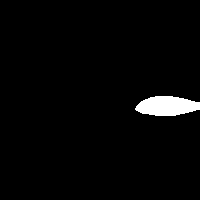
\includegraphics[height=0.18\textheight]{ch-methodology/figures/hca2-1}
}\hspace{0.15\linewidth}
\subfigure[$k=2$]{
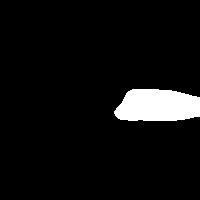
\includegraphics[height=0.18\textheight]{ch-methodology/figures/hca2-2}
}\\
\subfigure[$k=3$]{
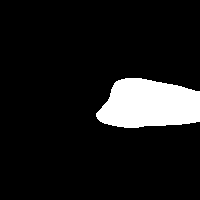
\includegraphics[height=0.18\textheight]{ch-methodology/figures/hca2-3}
}\hspace{0.15\linewidth}
\subfigure[$k=4$]{
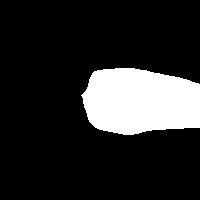
\includegraphics[height=0.18\textheight]{ch-methodology/figures/hca2-4}
}\\
\subfigure[$k=5$]{
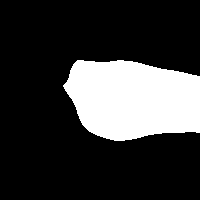
\includegraphics[height=0.18\textheight]{ch-methodology/figures/hca2-5}
}\hspace{0.15\linewidth}
\subfigure[$k=6$]{
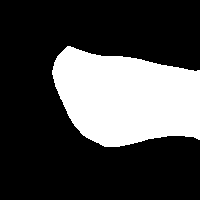
\includegraphics[height=0.18\textheight]{ch-methodology/figures/hca2-6}
}\\
\subfigure[$k=7$]{
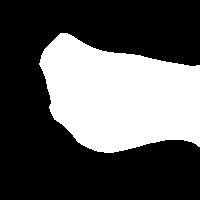
\includegraphics[height=0.18\textheight]{ch-methodology/figures/hca2-7}
}\hspace{0.15\linewidth}
\subfigure[$k=8$]{
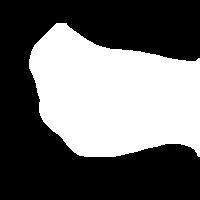
\includegraphics[height=0.18\textheight]{ch-methodology/figures/hca2-8}
}
\caption[$L^k$ of another sample from palm 1]{$L^k$ for $k=1,2,\dots,8$ of a 3D ROI from another palmprint sample from the same person as in Figure ~\ref{fig:methodology:hcalevels1}}
\label{fig:methodology:hcalevels2}
\end{figure}

\begin{figure}[htb]
\centering
\subfigure[$k=1$]{
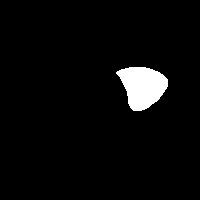
\includegraphics[height=0.18\textheight]{ch-methodology/figures/hca3-1}
}\hspace{0.15\linewidth}
\subfigure[$k=2$]{
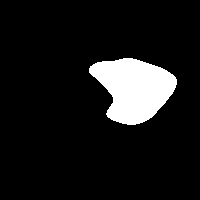
\includegraphics[height=0.18\textheight]{ch-methodology/figures/hca3-2}
}\\
\subfigure[$k=3$]{
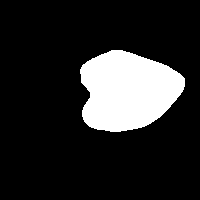
\includegraphics[height=0.18\textheight]{ch-methodology/figures/hca3-3}
}\hspace{0.15\linewidth}
\subfigure[$k=4$]{
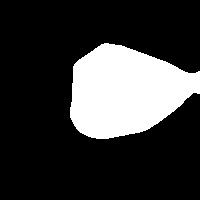
\includegraphics[height=0.18\textheight]{ch-methodology/figures/hca3-4}
}\\
\subfigure[$k=5$]{
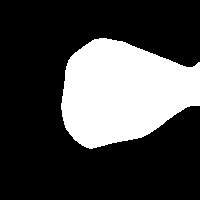
\includegraphics[height=0.18\textheight]{ch-methodology/figures/hca3-5}
}\hspace{0.15\linewidth}
\subfigure[$k=6$]{
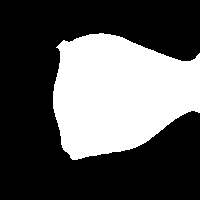
\includegraphics[height=0.18\textheight]{ch-methodology/figures/hca3-6}
}\\
\subfigure[$k=7$]{
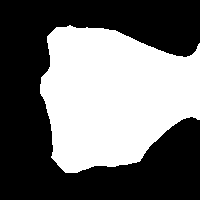
\includegraphics[height=0.18\textheight]{ch-methodology/figures/hca3-7}
}\hspace{0.15\linewidth}
\subfigure[$k=8$]{
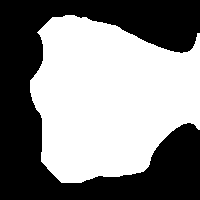
\includegraphics[height=0.18\textheight]{ch-methodology/figures/hca3-8}
}
\caption[$L^k$ of one sample from palm 2]{$L^k$ for $k=1,2,\dots,8$ of a 3D ROI from a palmprint sample from the a different person from that of Figure ~\ref{fig:methodology:hcalevels1}}
\label{fig:methodology:hcalevels3}
\end{figure}

\begin{figure}[htb]
\centering
\subfigure[$k=1$]{
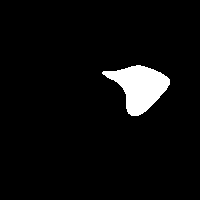
\includegraphics[height=0.18\textheight]{ch-methodology/figures/hca4-1}
}\hspace{0.15\linewidth}
\subfigure[$k=2$]{
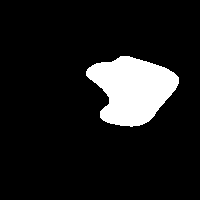
\includegraphics[height=0.18\textheight]{ch-methodology/figures/hca4-2}
}\\
\subfigure[$k=3$]{
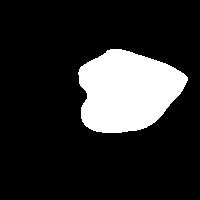
\includegraphics[height=0.18\textheight]{ch-methodology/figures/hca4-3}
}\hspace{0.15\linewidth}
\subfigure[$k=4$]{
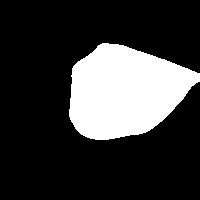
\includegraphics[height=0.18\textheight]{ch-methodology/figures/hca4-4}
}\\
\subfigure[$k=5$]{
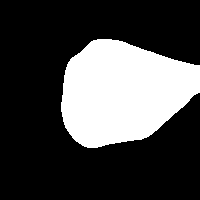
\includegraphics[height=0.18\textheight]{ch-methodology/figures/hca4-5}
}\hspace{0.15\linewidth}
\subfigure[$k=6$]{
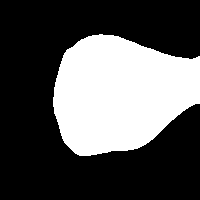
\includegraphics[height=0.18\textheight]{ch-methodology/figures/hca4-6}
}\\
\subfigure[$k=7$]{
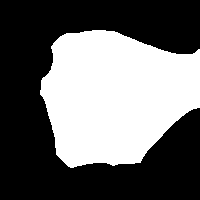
\includegraphics[height=0.18\textheight]{ch-methodology/figures/hca4-7}
}\hspace{0.15\linewidth}
\subfigure[$k=8$]{
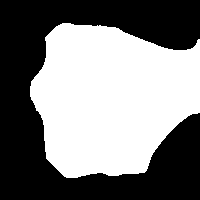
\includegraphics[height=0.18\textheight]{ch-methodology/figures/hca4-8}
}
\caption[$L^k$ of another sample from palm 2]{$L^k$ for $k=1,2,\dots,8$ of a 3D ROI from another palmprint sample from the same person as in Figure ~\ref{fig:methodology:hcalevels3}}
\label{fig:methodology:hcalevels4}
\end{figure}

Figure ~\ref{fig:methodology:hcalevels1} and ~\ref{fig:methodology:hcalevels2} shows the cross-sectional area feature from two samples collected from one palm. Figure ~\ref{fig:methodology:hcalevels3} and ~\ref{fig:methodology:hcalevels4} are extracted from two samples from another palm.
